\section{Evaluation} \label{sec:eval}

We compare the performance of \alg\ to the following multiprocessor algorithms: 
%\inred{
\begin{description}
\item[\pBMW]\cite{rojas2013efficient} -- parallel BMW,  
the best-in-class parallelization of a document-order top-k algorithm; 
\item[\pJASS]\cite{parallel-jass} -- a recent parallelization of the JASS~\cite{Lin:2015} score-order retrieval algorithm; 
\item[\pRA]-- a parallel implementation of RA;
\item[\sNRA]--  a shared-nothing  parallelization of NRA; and 
\item [\pNRA]-- a
na\"{\i}ve shared-state parallel implementation of NRA. 
\end{description}
%}
Although our primary focus is on  approximate 
algorithms, for completeness, we also experiment with their exact counterparts.
%
% We study all these algorithms in both exact and approximate variants -- the latter over a spectrum of heuristic parameters that strike different performance-vs-recall tradeoffs.  

{
%\inred{
In order to crystallize the comparison among  the core algorithms, 
we abstract away other contributors to the wall-clock  latency, e.g., index compression. 
As recent studies show, with the state-of-the-art compression techniques the impact 
of decompression on the end-to-end performance is marginal (e.g., up to $6\%$ surplus with the QMX-D4 compression~\cite{Lin:2017}).  Compression effectiveness of document-order vs score-order indexes is beyond the context of this paper.

We focus on disk-resident search indexes (most of the algorithms under study are of 
streaming nature, and hence CPU-bound; fitting the index in RAM does not affect 
their performance significantly). 
%}

In what follows, Section~\ref{ssec:setup} describes the experiment setup, 
Section~\ref{ssec:implementation} explains how the algorithms are 
implemented, and Section~\ref{ssec:results} presents our results.


\subsection{Experiment Setup}
\label{ssec:setup}

We study the algorithms in terms of query latency and throughput attainable at a single multi-core server. 
We use mid-tier industry-standard hardware -- a 12-core Intel Xeon E5620 with 24GB RAM and 1TB SSD drive. 

The benchmarking environment and the algorithms  are implemented in Java. 
A  \emph{benchmark driver} draws queries from an input queue and submits them to the algorithm being tested, which
% It runs the queries either one-by-one (latency mode) or in parallel (throughput mode).
%In both modes, the algorithm exploits 
uses a thread pool for intra-query parallelism. 
The driver controls the pool size. % by notifying the algorithm how many threads are available to it.
When testing latency, the thread pool is used by a single query. 
In the throughput evaluation mode, queries are scheduled first-come-first-served, 
and a new query is scheduled for execution (i.e., assigned threads) 
once  there are idle threads with no outstanding work from currently executing queries.
All queries scheduled for execution equally share the thread pool.

In all experiments, the appropriate index (either in id order or in score order)
is pre-built offline and stored on disk uncompressed as a collection of binary files, 
each storing a shard of data partitioned by term.  The benchmark environment memory-maps the content 
of these files via the MappedByteBuffer API~\cite{java-bytebuffer}.
Prior to each experiment, we flush the file system's page cache so all pages are physically read from disk during the experiment.


%such that the algorithm code can access the data identically to RAM. 
%The application code makes no attempt to optimize the disk access beyond the standard filesystem mechanisms 
%(e.g., caching of popular blocks). 

%\subsubsection{Datasets}
We  experiment with the TREC dataset, Category B ({\cw}09B), which is widely used for information retrieval research~\cite{ClueWeb09}. This dataset includes approximately 50M web documents and takes up roughly 30GB of original content, uncompressed.

\bigdataset{
two document corpora. The first  is 
}
\bigdataset{
The second corpus is a synthetic 10x scale-up of \cw, named \cwten, which we created to explore the algorithms' scalability 
with the dataset size. 
% \cwten\ is a superset of {\cw}09B.
The 450M synthetic documents in {\cwten\/} are generated as follows. Each document is a bag of words drawn from the original {\cw\/} dictionary 
(the order is immaterial for our document scoring function) 
%, see Section~\ref{ssec:scoring}) 
so that the number of occurrences of a term $t_i$ with an original 
global frequency rate of $F(t_i)$ is drawn from a geometric distribution with a stopping probability of $1-F(t_i)$. This  process preserves 
the  term frequency distribution of {\cw\/} in \cwten.
 }
 
% \inred{
We use the popular Lucene open-source search engine~\cite{lucene} for preprocessing the index to generate posting lists; this  includes text tokenization, posting list maintenance, 
and term statistics retrieval.
%}
We score documents using a standard tf-idf score function with document length normalization~\cite{Baeza-Yates:1999:MIR:553876}. 

We draw queries from the public AOL search log~\cite{aol}.
For each number of terms from $1$ to $12$, we independently sample $100$ queries of this length uniformly at random from the AOL log.
We also  experimented with a query log of another commercial web search engine; this experiment  
produced statistically similar results, and so we omit them here.  

We use  $k=1000$, {based on the assumption that simple tf-idf retrieval is the first phase of multi-stage ranking, 
which may require large values of $k$ for effectiveness~\cite{Wang:2011}. (Indeed, Crane et. al.~\cite{Crane:2017} report
that the classical AP and RBP quality metrics are close to optimal with this choice of $k$, for multiple datasets.)}  
Experiments with $k=100$ produced qualitatively similar results.% {\inred{which we omit for lack of space}}.

\remove{
\subsubsection{Document Scoring}
\label{ssec:scoring}
For document evaluation, we apply a simple tf-idf score function with document length normalization~\cite{Baeza-Yates:1999:MIR:553876} as follows:
\[ \textit{ts}(D, t_i) \triangleq \frac{\textit{idf}(t_i) \cdot \textit{freq}(D, t_i)}{\sqrt{|D|}},\]
where \textit{freq}$(D, t_i)$ is the frequency of term $t_i$ in document $D$,
$\textit{idf}(t_i)$ is  the inverse document frequency of term $t_i$,
and $|D|$ is the number of tokens in $D$. 
}

\subsection{Implementation}
\label{ssec:implementation}

%All algorithms store 
Posting lists are stored as contiguous uncompressed arrays;  {\pRA} also stores 
its secondary index (document id to position in the posting list mapping) in the same form. 
Term scores (namely, tf-idf) are stored in the posting lists as integers, scaled by $10^6$ and rounded as in~\cite{Bortnikov:2017}. 
Using integer arithmetics instead of floating-point significantly speeds up document evaluation. 

The specific algorithm implementations are as follows.

\subsubsection{State-of-the-art parallel search algorithms}

\paragraph{\pBMW}
Our implementation of {\pBMW} closely follows the description in~\cite{rojas2013distributing}. The algorithm partitions the execution of the 
sequential BMW~\cite{Ding:2011} among multiple threads. Each thread handles a distinct subset of documents, and computes a local top-k 
result. The algorithm then merges the partial results to obtain the final top-k. 
%See Section~\ref{sec:related} for detail.

Similarly to \alg, \pBMW's threads obtain jobs from a common job queue. Here, a job defines a range of document ids to scan. 
We set the number of jobs to be twice the number of worker threads, and assign equal-size ranges to all threads.  
This partition results in well-balanced execution in which the whole worker pool is utilized 
most of the time. 

Each thread maintains a thread-local heap with the current top-k documents. (We also experimented with a shared heap and 
got inferior results; a similar finding was reported in~\cite{rojas2013distributing}.)
Similarly, each thread $T$ maintains a local threshold $\Theta_T$ for filtering heap insertions; 
$\Theta_T$ is \emph{at least} the lowest score in the local heap, but may be higher thanks to the progress of other threads.  
%Specifically, threads benefit from each other's progress via a shared $\Theta$ variable. 
Thread $T$ periodically compares $\Theta$ to its local $\Theta_T$, and promotes the smaller of the two to $\max(\Theta_T, \Theta)$. 
This way,  slower workers catch up with  faster ones.

\pBMW\
%, which is applied to a segment of posting lists, further 
splits posting list segments into blocks, and uses block-level
statistics to prune the search~\cite{Ding:2011}. We experimented with multiple block sizes and selected $64$, 
which yielded the best performance.
% In 
The approximate version's pruning aggressiveness is  controlled by  a parameter 
$f \geq 1$, which multiplies $\Theta$ to relax the threshold for score upper bounds~\cite{Broder:2003}. For $f=1$, the algorithm is exact.

%\inred{
\paragraph{pJASS}
Our implementation of pJASS  follows the description in~\cite{parallel-jass}. It traverses all posting lists in parallel, in score order, and accumulates the encountered scores 
per-document in  \emph{docMap}. Each document is protected by a lock, and a thread that encounters a document locks it, adds the partial score from the term it traversed, and then unlocks it.
The algorithm stops after a predefined fraction of postings (denoted $p$) are scanned.
%}

\subsubsection{Parallel TA variants}

\sNRA\ is a shared-nothing parallelization of NRA, where the index is partitioned to $12$ shards by document id. 
Each thread finds the top-k documents in its shard by running NRA independently with thread-local data structures. 
When all threads complete, their lists are merged and the global top-k documents are kept.  

\pNRA\ is a na\"{\i}ve shared-state parallelization of NRA that does not employ \alg's optimizations. 
Namely, it uses a shared document map, which it does not clean, and updates the term
upper bounds upon every document evaluation. As in \alg, a dedicated task checks the stopping condition.
(Distributed stopping detection yielded worse results).

\remove{
Similarly to {\pNRA} and \alg, {\pRA} traverses the posting lists in segments, using a job queue. 
In contrast with them, {\pRA} computes complete document scores using its secondary index, 
instead of maintaining partial scores. 
Note that {\pRA} is the only studied algorithm that exercises random access to persistent storage.  
} 

{\pRA} maintains its results in a shared heap (experiments did not show any advantage to using local heaps).
Note that the algorithm's multiple worker threads may encounter postings of the same document independently, 
and consequently score that document and try to insert it into the heap multiple times. The implementation guarantees 
the uniqueness of insertion (only the first one takes effect).

%{\pRA} halts execution if no new results have been produced for $\Delta$ time ($\Delta=\infty$ means the result is exact). 
Since RA's stopping detection is lightweight, we do not dedicate a task to it. Instead, all workers check the  
\RAStop\ condition and monitor the time elapsed since the last heap update, and notify each other if they 
decide to stop.
%A thread that detects that the algorithm can stop notifies all threads.



\subsection{Results}
\label{ssec:results}

For an algorithm A, we consider the following variants: exact (denoted A\ex), high-recall (denoted A\hi), and
low-recall (denoted A\lo). Note that the approximate algorithms' parameters ($\Delta$ and $f$) affect the recall
but do not directly control it; our high recall instances are ones that empirically achieve a  recall of $97\%$ or 
higher.
\bigdataset{ 
for both datasets.
}
%\cw\/ and \cwten. 

\remove{
We evaluate the query processing latency and throughput 
induced by the candidate algorithms, 
for $k=1000$. 
(Experiments with $k=100$ produced qualitatively similar results).
 }


\subsubsection{Exact Algorithms}

\begin{table}[tbp]
\begin{center}
\begin{tabular}{| c | c | c | c | c | c|}
\hline
  Sparta & \pNRA & \sNRA & \pRA & \pBMW & pJASS \\ \hline
  860 & 13\!,291 & 5\!,553 & 480 & 750 & 54\!,343 \\ \hline
\bigdataset{
 ClueWebX10 & 12\!,010 & $90\!,000+$ & 56\!,223 & $7\!,410$ & $10\!,210$ \\
}
\hline
\end{tabular}
\end{center}
\caption{Average query latency (in ms) of 12-term queries with exact algorithms using 12  threads. 
None of the algorithms meets  real-time SLAs. }
\label{tab:safe-latency}
\end{table}

Our first experiment shows that none of the exact algorithms meets a real-time SLA for  verbose queries. 
Table~\ref{tab:safe-latency} depicts the mean processing latencies of 12-term queries with 12 worker 
threads (i.e., a single query fully exploits the multi-core CPU). 
\bigdataset{
Most of the algorithms complete within 
%500 ms to 
1 second for on the {\cw} dataset, but run for many seconds on \cwten. 
{\pRA} is the fastest algorithm in this setting, whereas
\pNRA\/ is much worse than the other algorithms. Its average latency exceeds 
13 seconds on \cw\/ and 1.5 minutes on \cwten.
} 

We will revisit the algorithms' execution dynamics -- namely, how fast they accrue their results -- 
as we study approximate algorithms in the sequel. 
 
\subsubsection{Approximate Algorithms}
 
With  exact instances of all  algorithms failing to match  real-time requirements, we turn to focus on the approximate instances. 
We parameterize \alg, \pRA, \pNRA, and \sNRA\/ with $\Delta=10$ ms. 
This yields high recall in all four algorithms,  and satisfactory performance (meeting SLA requirements) in \alg. 
We instantiate \pBMW\/ with $f=5$ for high recall and $f=10$ for low recall.  
{Finally, \pJASS\/ is instantiated with $p=0.005$ for low recall and $p=0.02$ for high recall (using $p=0.1$, as suggested, e.g., 
in~\cite{Crane:2017}, produced unacceptably high latencies).

{\bf Accuracy.\ } Table~\ref{tab:recall-mrr-distance} depicts the empirical accuracy results for 12-term queries. 
%We see that the MRR-distance is high for the high-recall algorithms, 
%metric is closely correlated with recall 
%e.g., \alg\hi\/ yields $99\%$ recall and $0.002$ MRR-distance on \cwten. That is, these 
%algorithms not only  retain a large fraction of the true results, but also succeed in retaining the highest ranked ones. 

\remove{
This result is particularly interesting for \alg, which only computes partial scores. In practice, these scores are very close to the complete ones. 
In our experiments, on average, $93\%$ of the top-k documents have a correct score at the end of the execution. The average Pearson correlation
 between the correct scores and the partial scores is $0.999$.%, whereas the average Kendall's $\tau$ rank correlation is $0.86$. 


Summing up, under certain parameter choices the approximate algorithms achieve very high accuracy. We now focus on their performance. 
}
  
\begin{table*}[htbp]
\centering
\begin{tabular}{| c | c | c | c | c | c | c | c |}
\hline
   \alg\hi &  \pRA\hi & \pNRA\hi & \sNRA\hi & \pBMW\hi & \pBMW\lo & \pJASS\hi & \pJASS\lo \\ \hline
\bigdataset{  \cw & }
   97.5\%  &  98.5\%  & 98.5\%  & 99\%   & 97.5\% & 80\%  & 96\% & 93\%
  % 97.5\% / 0.004 &  98.5\% / 0.002 & 98.5\% / 0.002 & 99\% / 0.001  & 97.5\% / 0.009 & 80\% / 0.048 
  \\ \hline
\bigdataset{
  \cwten & 
  99\%  & 99\%  & 99\%  & 99\%  & 97\%  & 79.9\%  
  \\ \hline
  }
  % 99\% / 0.002 & 99\% / 0.001 & 99\% / 0.001 & 99\% / 0.001  & 97\% / 0.009 & 79.9\% / 0.099 
\end{tabular}
%\caption{Recall / MRR-distance induced by the approximate algorithms for 12-term queries.}
\caption{Recall of approximate algorithms for 12-term queries.}
\label{tab:recall-mrr-distance}
\end{table*}

{\bf Latency.\ } 
Figure~\ref{fig:terms-scaling} depicts the scaling of single-query latency of the approximate algorithms  
as the number of terms scales from $1$ to $12$. The number of workers in each test 
is equal to the number of terms (for \alg, \pRA, and \pNRA, this allows maximal parallelism). 

Figure~\ref{fig:terms-scaling-high-avg} and Figure~\ref{fig:terms-scaling-high-95} present, respectively, the  mean and  
$95\%$ latencies of queries\bigdataset{ on  {\cw}} for \alg\hi\ and the rest of the high-recall algorithms. The latter captures the so-called ``tail latency'' of 
the slowest $5\%$ of the queries. Figure~\ref{fig:terms-scaling-low-avg} and Figure~\ref{fig:terms-scaling-low-95} present the same for \alg\hi\ and the low-recall algorithms.

\bigdataset{
;  Figure~\ref{fig:terms-scaling}(c) depicts the mean latency
for \cwten.
}
%
\alg\/ outperforms its competitors (guaranteeing either high or low recall) on all query sizes. The margin is especially big for verbose queries
($5+$ terms). \alg's average query latency scales perfectly, 
remaining below $180$ ms for all query lengths.
\bigdataset{
 for both \cw\/ and \cwten.  
}
%In other words, \alg's result set solidifies after processing 
%a similar number of postings, 
% even when the overall index size grows $10$x. 
Its  $95\%$ latency is below $500$ ms. 


\begin{figure*}[tbh]
\centering
\begin{tabular}{ccc}
      \begin{subfigure}[t]{0.4\textwidth}
         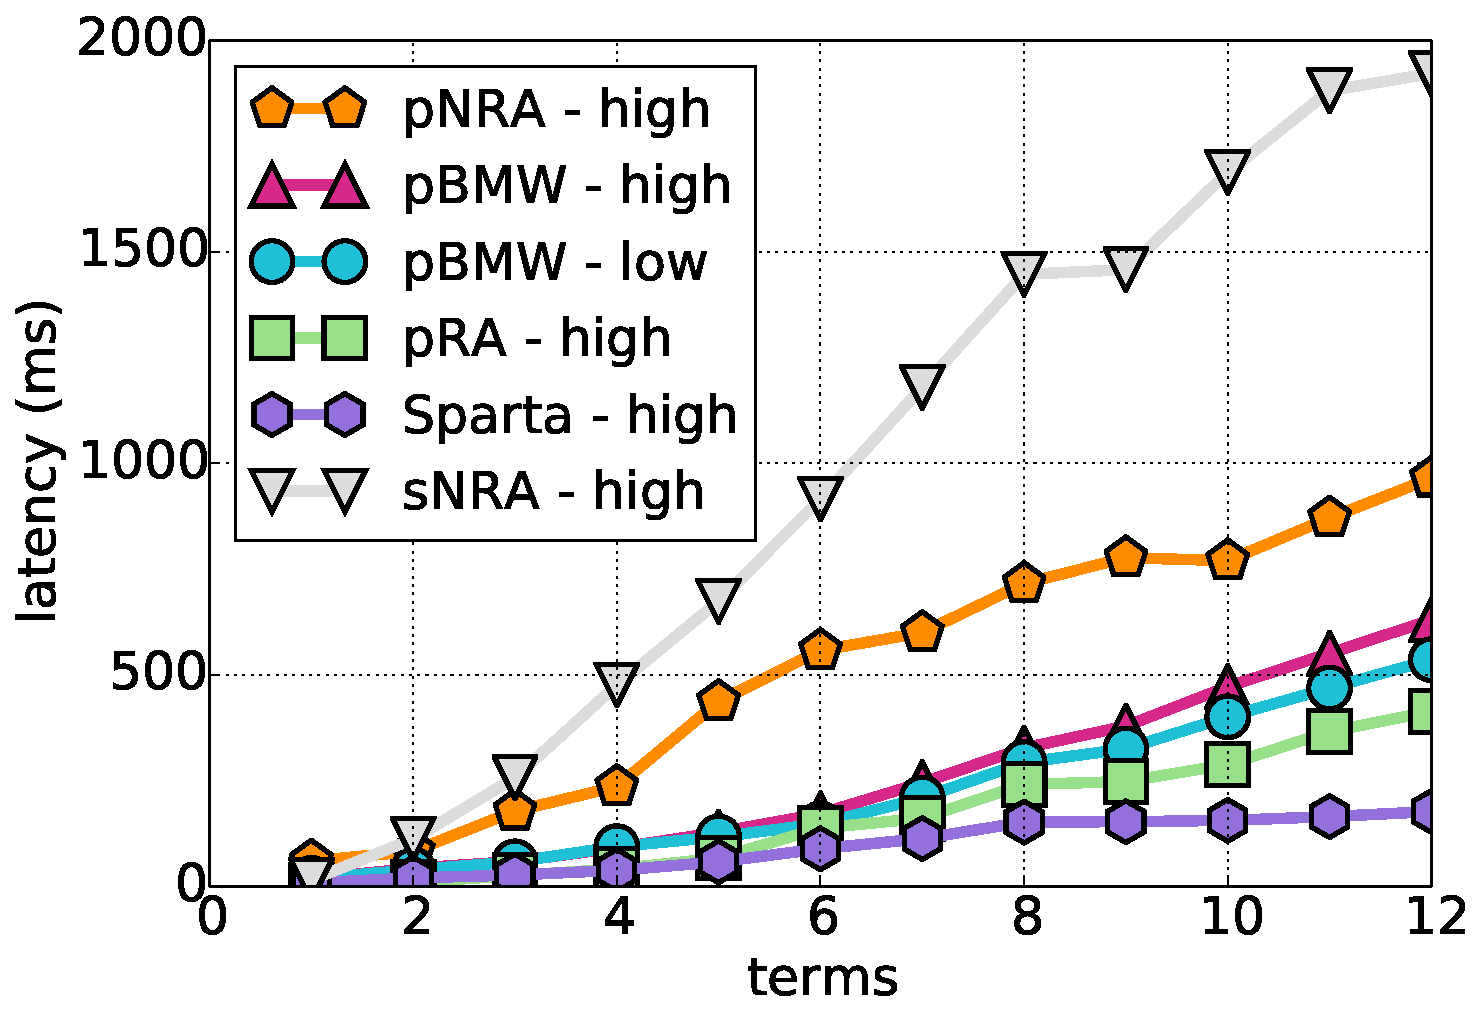
\includegraphics[width=\textwidth]{figures/latency_12threads_clueweb.pdf}
        \caption[]{Average\bigdataset{, \cw} - high recall algorithms}
        \label{fig:terms-scaling-high-avg}
      \end{subfigure}     

	\begin{subfigure}[t]{0.4\textwidth}
    	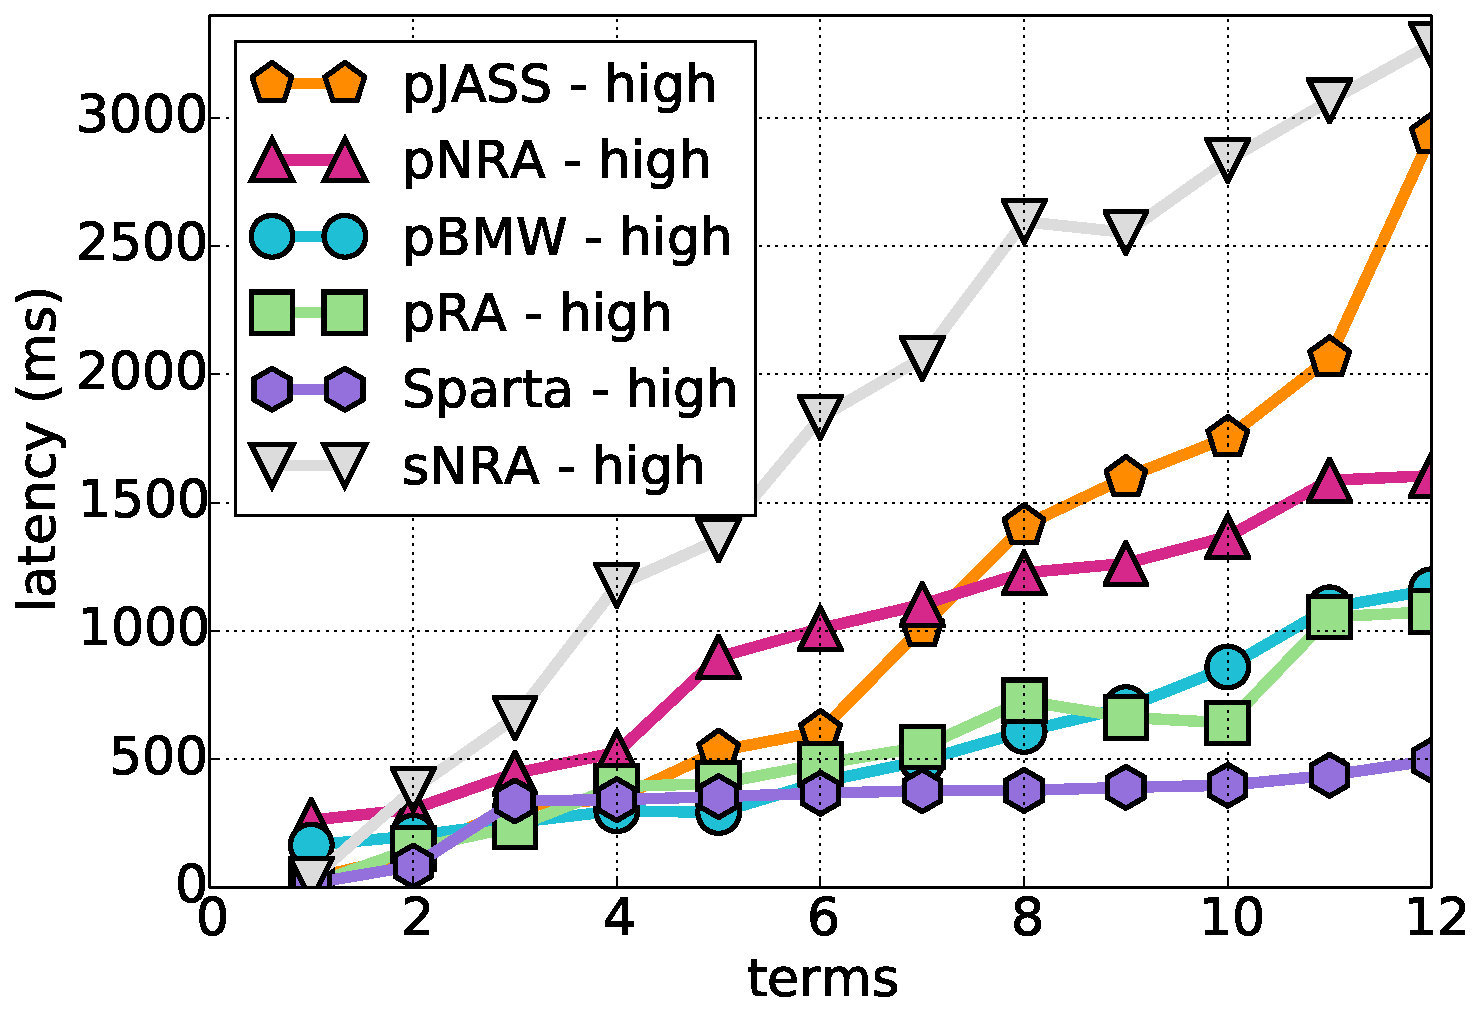
\includegraphics[width=\textwidth]{figures/latency_95th_percentile_clueweb.pdf}
	\caption{95\%\bigdataset{, \cw} - high recall algorithms}
	\label{fig:terms-scaling-high-95}
    \end{subfigure} 
    
\end{tabular} 
\begin{tabular}{ccc}
    
          \begin{subfigure}[t]{0.4\textwidth}
         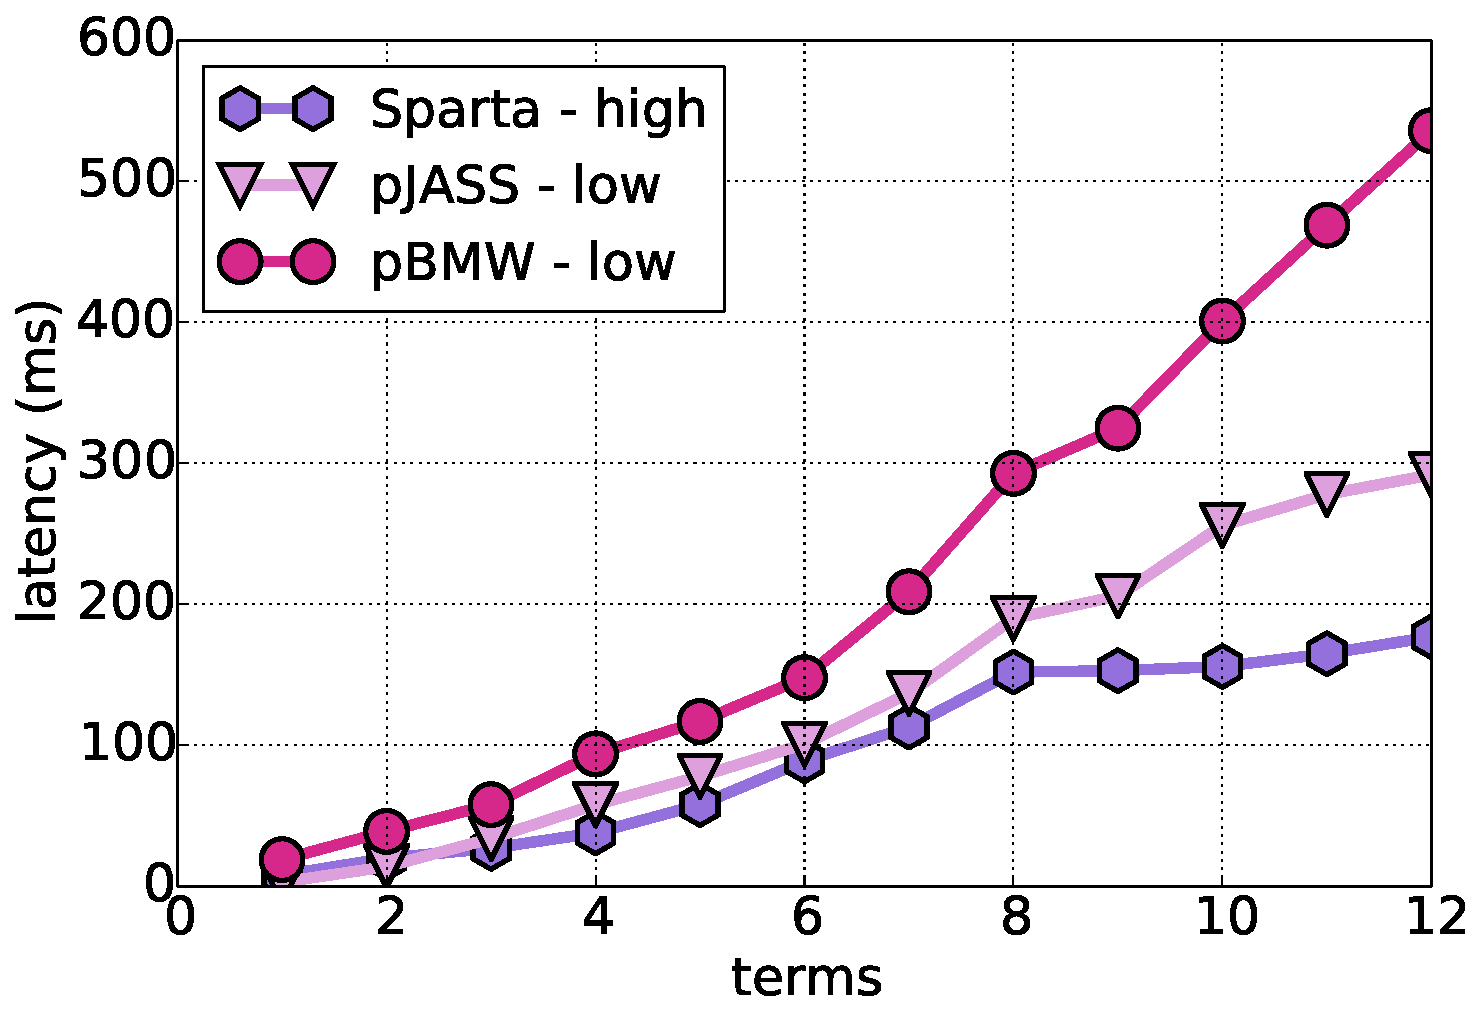
\includegraphics[width=\textwidth]{figures/latency_high_low_12threads_clueweb.pdf}
        \caption[]{Average\bigdataset{, \cw} - low recall algorithms}
        \label{fig:terms-scaling-low-avg}
      \end{subfigure}     

	\begin{subfigure}[t]{0.4\textwidth}
    	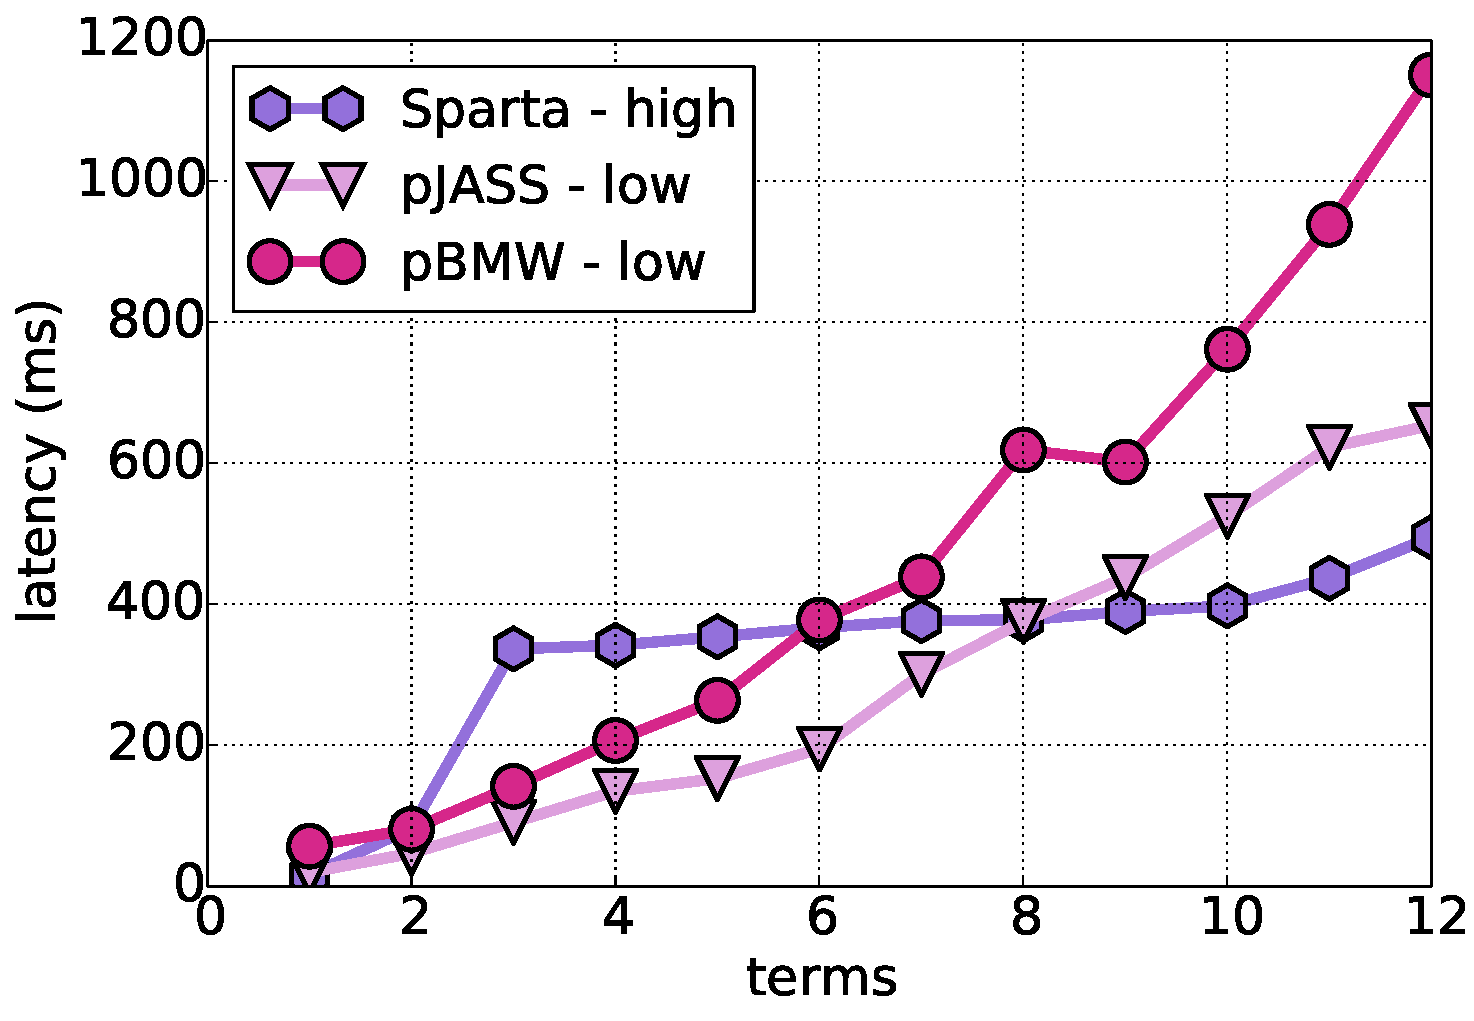
\includegraphics[width=\textwidth]{figures/latency_95th_percentile_high_low_clueweb.pdf}
	\caption{95\%\bigdataset{, \cw} - low recall algorithms}
	\label{fig:terms-scaling-low-95}
    \end{subfigure} 

\bigdataset{
    \begin{subfigure}[t]{0.3\textwidth}
    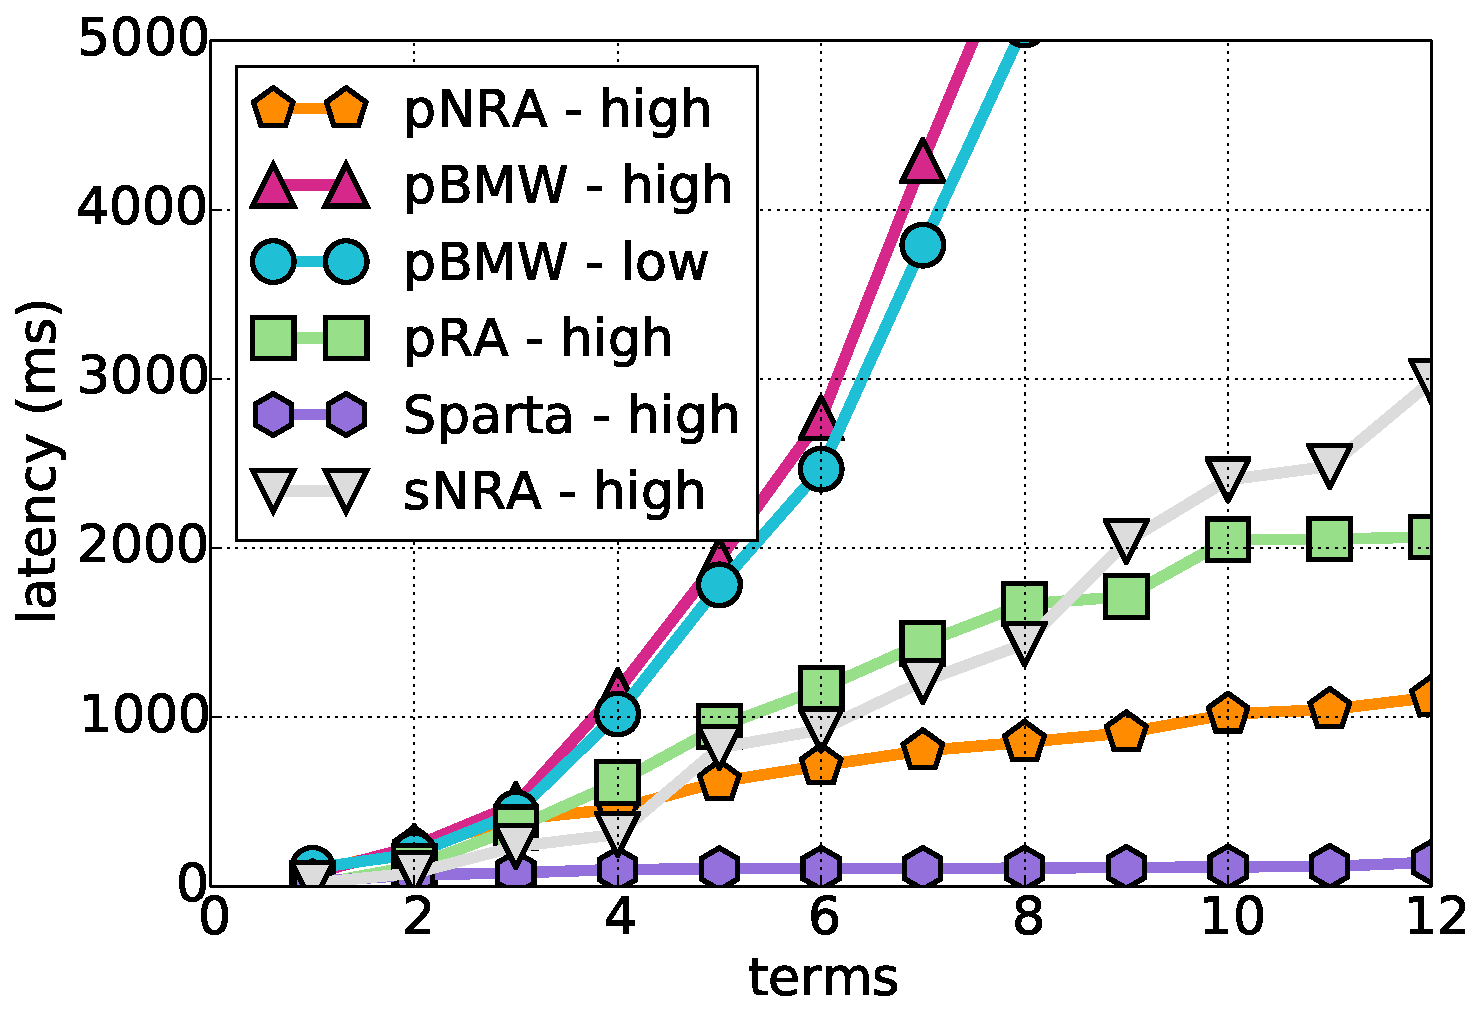
\includegraphics[width=\textwidth]{figures/latency_12threads_cluewebX10.pdf}
	\caption{Average, \cwten}
    \end{subfigure}  
    }
    
\end{tabular}
\caption{Top-k ($k=1000$) query latency scaling with the number of query terms. 
The intra-query parallelism is equal to the number of terms in all algorithms. Figures \ref{fig:terms-scaling-high-avg}-\ref{fig:terms-scaling-high-95} compare \alg\hi with the high recall algorithms and figures \ref{fig:terms-scaling-low-avg}-\ref{fig:terms-scaling-low-95} compare \alg\hi with the low recall algorithms}
\label{fig:terms-scaling}
\end{figure*}

\commentOut{
\begin{figure}[tbh]
\centering
\begin{tabular}{ccc}
      \begin{subfigure}[t]{0.3\textwidth}
         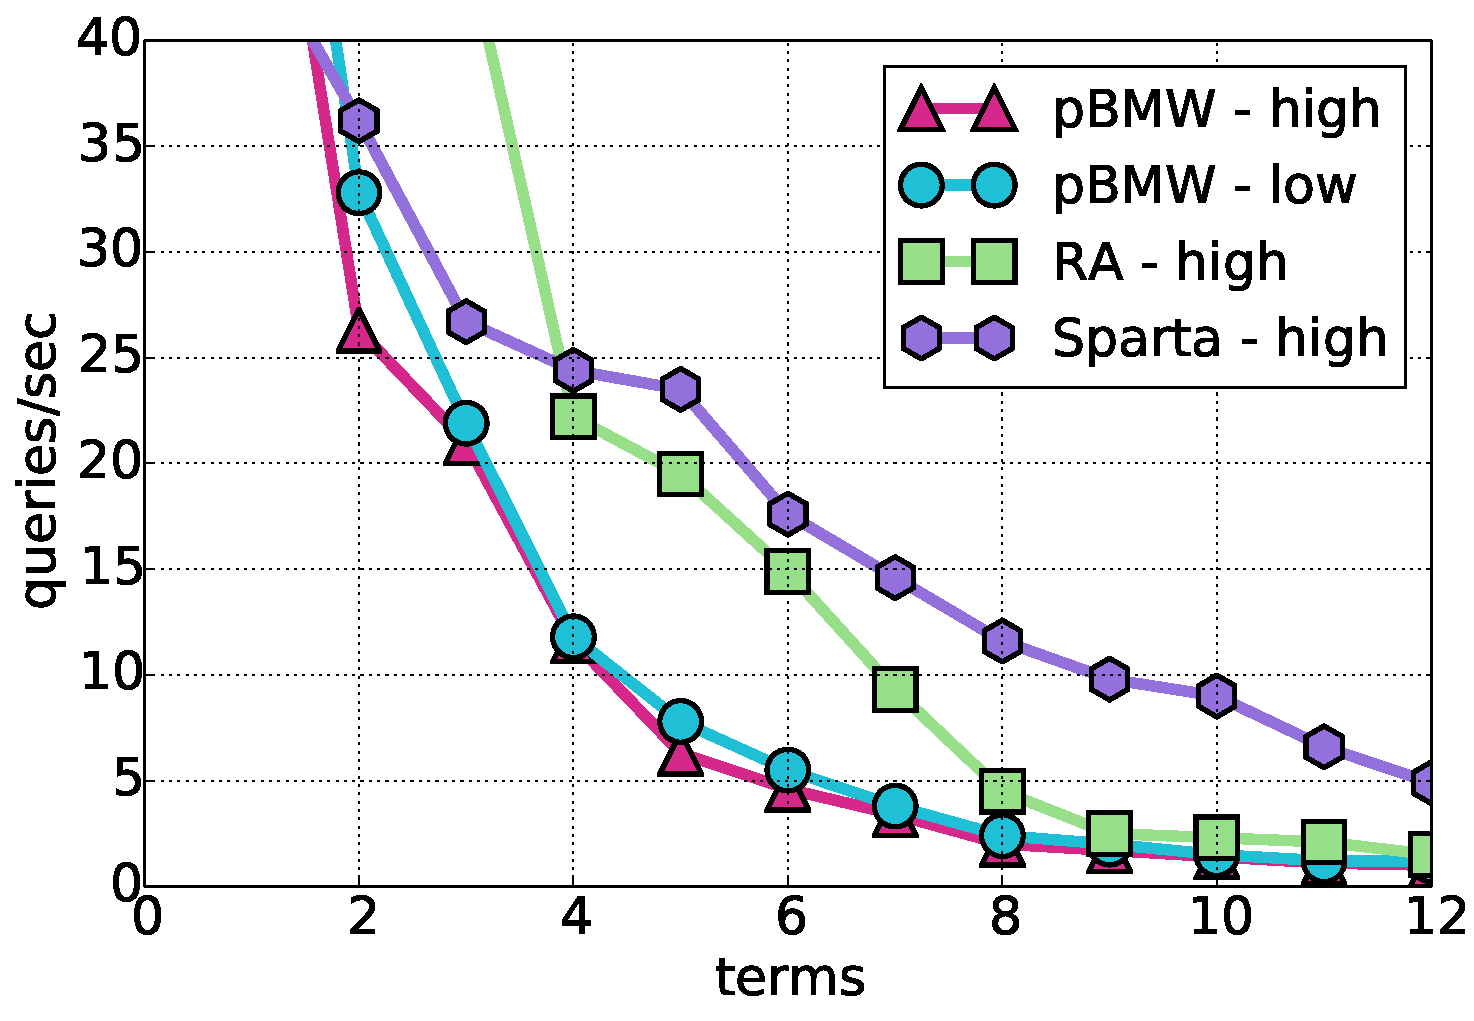
\includegraphics[width=\textwidth]{figures/throughput_12threads_clueweb.pdf}
      \end{subfigure}      
\end{tabular}
\caption{Top-k query throughput scaling with the number of query terms. The intra-query parallelism 
is equal to the number of terms in all parallel algorithms.}
\label{fig:throughput-scaling}
\end{figure}
}


In contrast, \pRA\/ exhibits much weaker scalability. For example, for $12$-term queries it is slower than \alg\
by more than $2$x. 
\bigdataset{
when applied to \cw, and by more than $10$x on \cwten. 
}
We explain this by the cost of evaluating the complete 
document scores in \pRA, which forces  intensive access to the secondary index. This translates to volumes of random 
I/O that cannot be sustained even with modern SSD hardware. Note that this trend is the reverse of the one observed for \pRA\ex, 
which outperforms \alg\ex\/ (Table~\ref{tab:safe-latency}). That is, \alg\/ spends much more work than \pRA\/ 
in order to collect the remaining $2.5\%$ of the exact result set. We revisit this phenomenon  below. 

\remove{
As an aside, note that \pRA\/ scales somewhat better if its whole working set fits into memory. 
However, this is seldom the case when diverse queries are applied to a large index.
%, e.g., when the same small set of queries is evaluated over and over again. 
%This use case is of limited interest.  
%besides, it does not manifest with the \cwten\/ dataset in statistically significant way. 
} 

We see that both
\pBMW\ and \pJASS\
%the best-in-class algorithm in the literature, 
fail to match \alg's speed. For example, for 12-term queries, 
\pBMW\hi\/ completes  within $630$ ms on average, 
\bigdataset{
on \cw, and within as long as $9.9$ seconds on \cwten. 
} 
\pBMW\lo, 
which sacrifices $20\%$ of the recall for performance, only succeeds to improve this latency by $10\%$ to $15\%$, 
\pJASS\hi\ completes  after more than a second on average, and \pJASS\lo\ completes  within $292$ ms on average.

\bigdataset{
On \cw, 
}
The shared-nothing and unoptimized parallelization of NRA are weaker than all other alternatives:
\pNRA's  average latency for 12-term queries is $1$ second, and \sNRA's is $1.7$ seconds. 
On the larger dataset, \pNRA\ and \sNRA\ are still poorer than \alg, but perform better than \pBMW. 
This is thanks to the high scalability and early-stopping nature of the approximate NRA approach.
These results emphasize the necessity of sharing information among threads (unlike \sNRA) on the one hand,
and the importance of \alg's locality optimizations, (which are missing in \pNRA), on the other. 
Specifically, the background cleaning and local copies of \DMap\ and the lazy updates of \emph{UB} allow \alg\ to benefit from 
local access to data that resides in hardware caches. 
We omit \pNRA\/ and \sNRA\/ from further discussion. 

\begin{figure}[hbt]
\centering
\bigdataset{
\begin{tabular}{ccc}
      \begin{subfigure}[t]{0.4\textwidth}
      }
         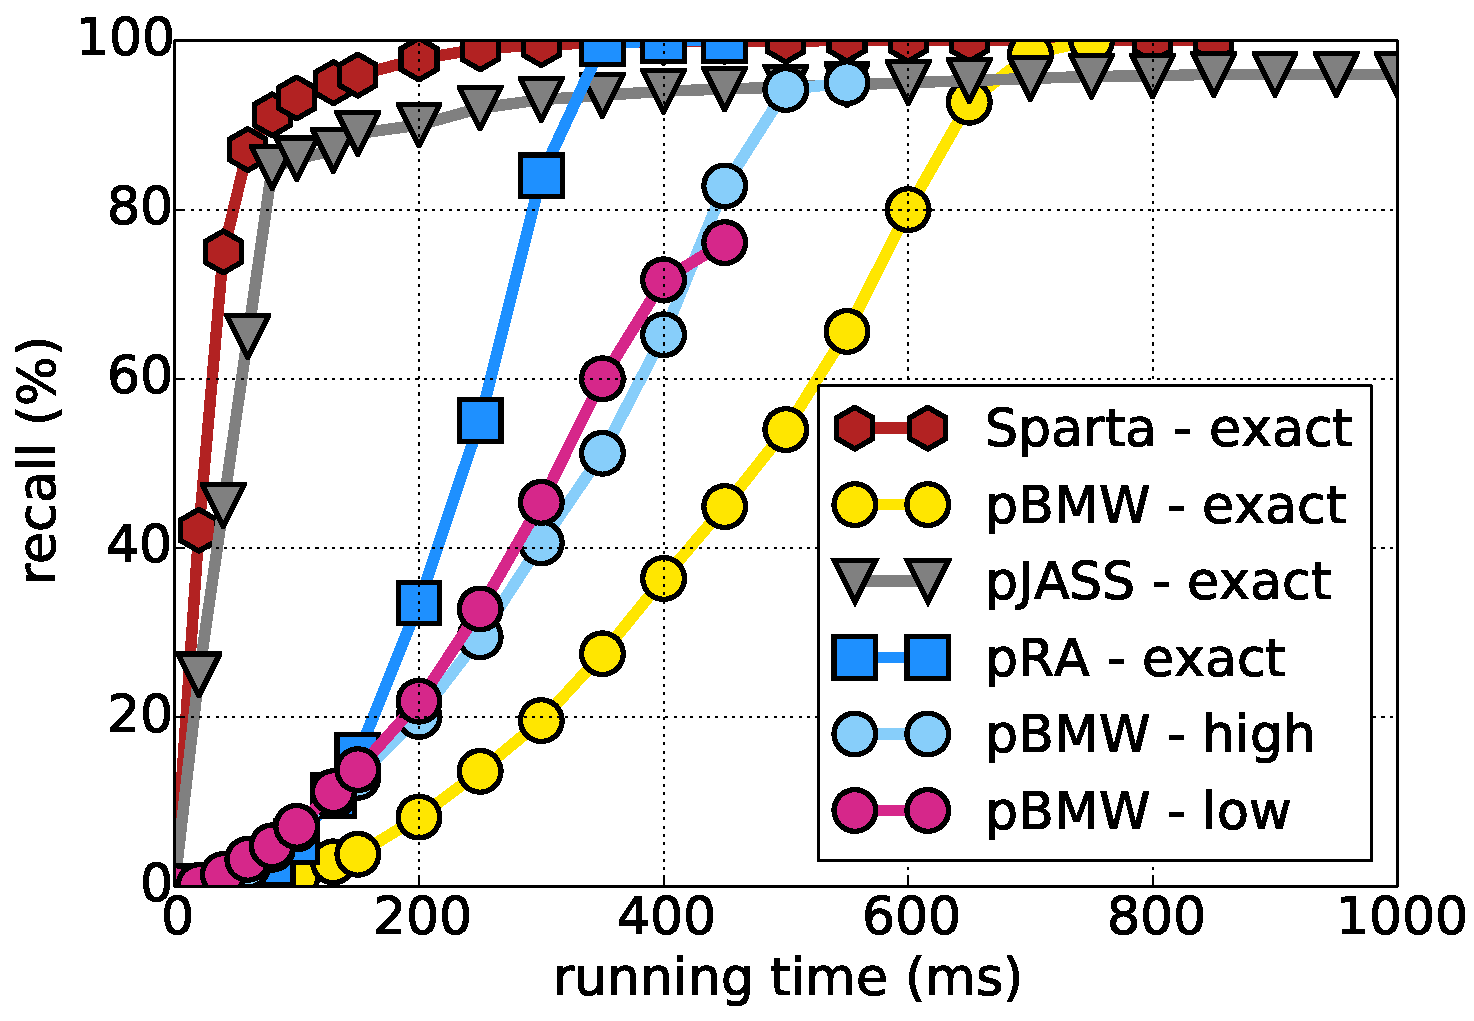
\includegraphics[width=0.4\textwidth]{figures/cumulative_12threads_clueweb.pdf}
\bigdataset{
        \caption[]{ClueWeb}
        \label{fig:dynamics-clueweb}
      \end{subfigure} 
    
& 
	\hspace{0.1\textwidth}
& 

      \begin{subfigure}[t]{0.4\textwidth}
      	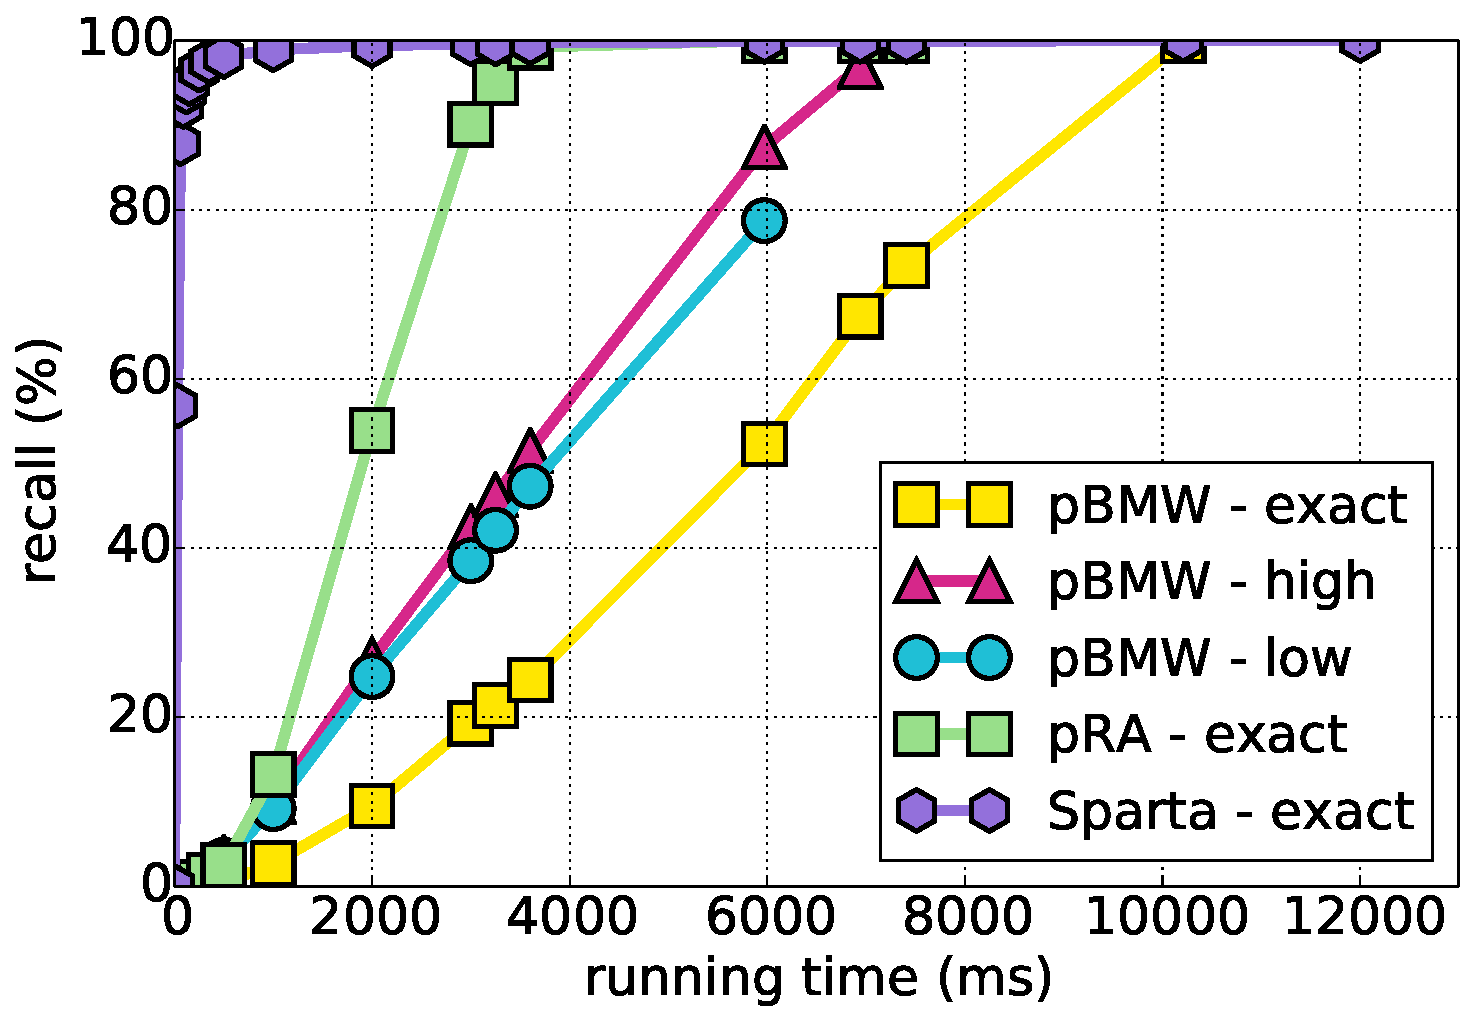
\includegraphics[width=\textwidth]{figures/cumulative_12threads_cluewebX10.pdf}
	    \caption{ClueWebX10}
	\label{fig:dynamics-cluewebX10}
      \end{subfigure}  
\end{tabular}
}
       \caption{Recall dynamics with elapsed time, for 12-term queries, with 12 worker threads.}
       \label{fig:dynamics}
\end{figure}

{\bf Recall dynamics.\ } 
In order to understand how the top-k results get accrued by the different algorithms, we zoom in on the dynamics of query 
recall over the running time. We focus on 12-term queries in a 12-worker configuration. The results are presented in 
Figure~\ref{fig:dynamics}\bigdataset{
(a) and Figure~\ref{fig:dynamics}(b) for the \cw\/ and \cwten\/ datasets, respectively 
}.
Because the approximate versions of \alg\, \pRA\ and \pJASS\ are  identical to the respective exact versions until they stop, 
we show the dynamics of the exact versions only.  The same is not true for \pBMW, where $f$ impacts the algorithm's results from the outset.
Hence, we show the dynamics of all three instances of \pBMW. 
%In the exact algorithms's curves, the rightmost data point corresponds to the exact algorithm's completion time.   

We see that \alg's recall growth is the fastest. For instance, it surpasses $80\%$ recall in less than $50$ ms, 
and $90\%$ recall in less than 100. But over time, its returns  diminish, and most of the work becomes unproductive. Whereas
\pRA\/ takes much longer to converge because it needs to fully score each encountered document,  its concluding phase is faster because 
most relevant documents   have complete  scores. 
\pBMW\/ scans the postings in the order of document ids, which is unrelated to document scores, and hence accumulates the true hits 
at a near-linear rate. Obviously, the convergence rate of \pBMW\hi\/ and \pBMW\lo\/ is faster than that of \pBMW\ex. For both datasets, the first 
two accrue results at similar rates until \pBMW\lo\/ stops at approximately $80\%$ recall.
\pJASS's behavior  is similar to \alg's, but it is a bit slower and does not reach a $100\%$ recall within a minute of execution.

%Figure~\ref{fig:terms-scaling}(c) zooms in on \alg's performance versus other variants of NRA: AllPar -- a na\"{\i}ve parallelization  (without the initial sequential phase),  Seq -- a sequential implementation, and SharedState -- a version of \alg\ that does not use local \TMap\/s. Neither of the first two scales with real-time latency. Interestingly, AllPar is slower than Seq, underscoring the importance of aggressive pruning prior to starting the concurrent execution. SharedState is substantially faster, but fails to utilize the hardware cache efficiently due to lack of locality. It thus lags behind \alg\/ by approximately $35\%$ for long queries. 
{\bf Parallelism.\ } 
%We next study the scaling of query latency with  intra-query parallelism. 
We next consider  $12$-term queries with a number of threads varying from $1$ to $12$. 
The results appear in Figure~\ref{fig:threads-scaling}\bigdataset{(a) (for \cw) and Figure~\ref{fig:threads-scaling}(b) (for \cwten). The latter depicts only \alg\/ and \pRA\/ 
because none of the \pBMW\/ instances scales close to real-time performance}.  
The left-most data point in each curve refers to the performance of 
the respective sequential algorithm.

\alg\ requires some level of parallelism in order to achieve real-time speed, e.g., its sequential
latency 
\bigdataset{
on \cw\/  
}
is $840$ ms, which is  above typical SLA requirements. Most of the gain is achieved at low-parallelism levels (2 threads suffice). 
On the other hand, for \pBMW, much higher parallelism is essential -- its latency is inversely proportional to the number of threads. Thus, \alg\ is not only faster 
than \pBMW, but also requires less resources, which benefits throughput as we next show.
%offers the system designer a latency-throughput tradeoff if some slack in latency can be tolerated. 

\begin{figure}[tbh]
\centering
\bigdataset{
\begin{tabular}{ccc}
      \begin{subfigure}[t]{0.4\textwidth}
}
         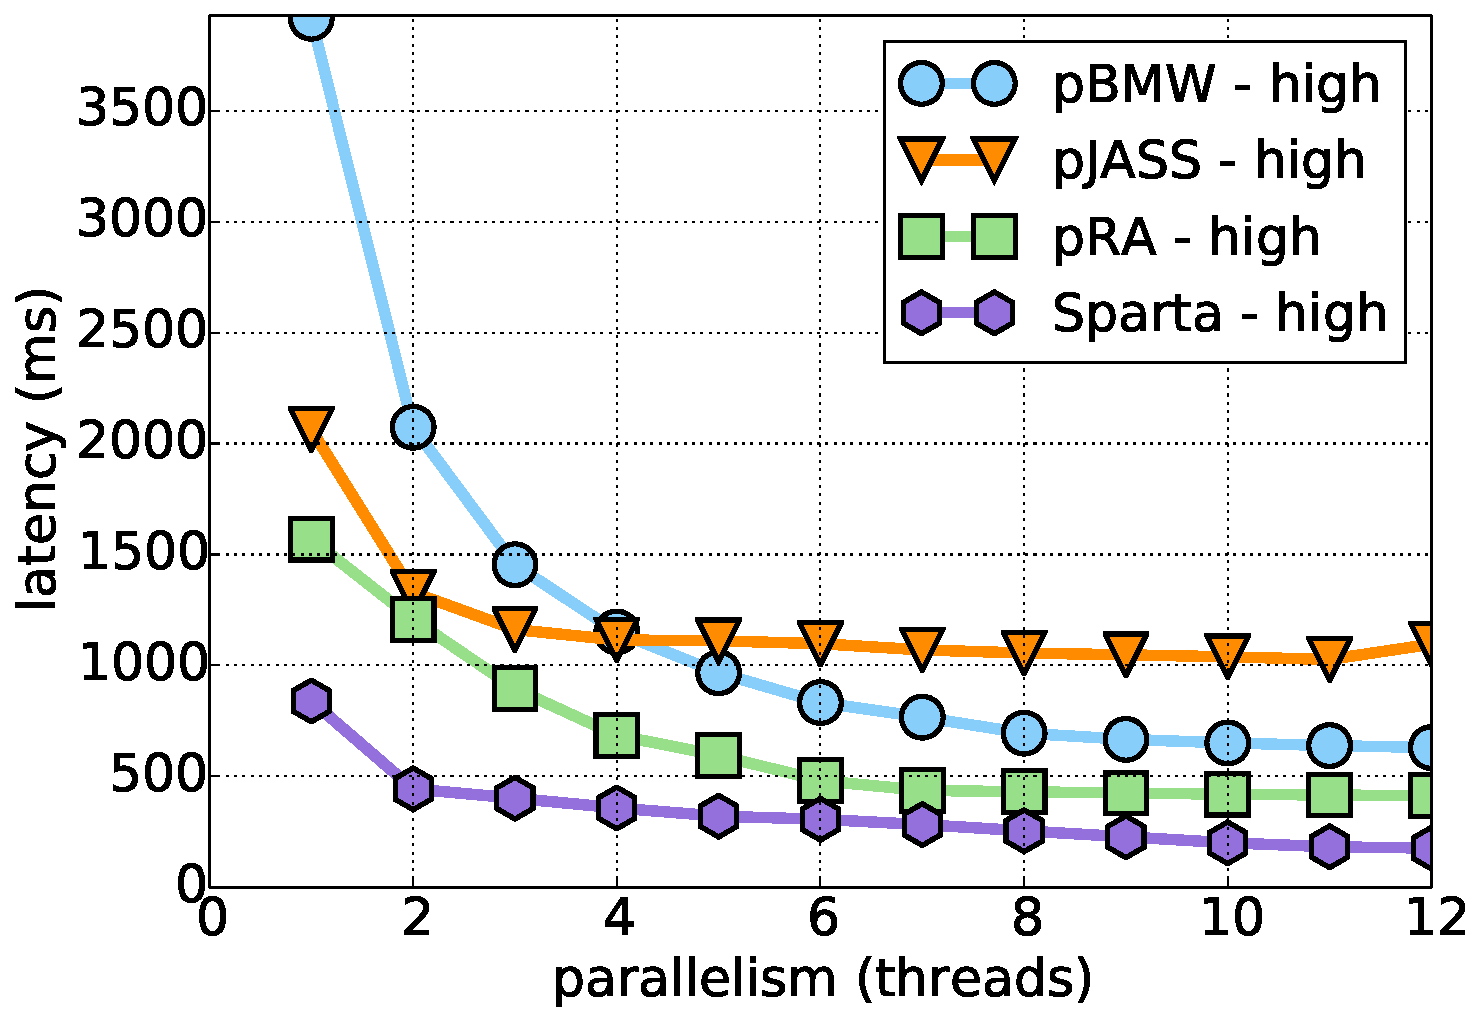
\includegraphics[width=0.4\textwidth]{figures/latency_12terms_clueweb.pdf}
\bigdataset{
        \caption[]{ClueWeb}
    %    \label{fig:varying-threads-6-terms}
      \end{subfigure} 
& 
	\hspace{0.1\textwidth}
& 
      \begin{subfigure}[t]{0.4\textwidth}
      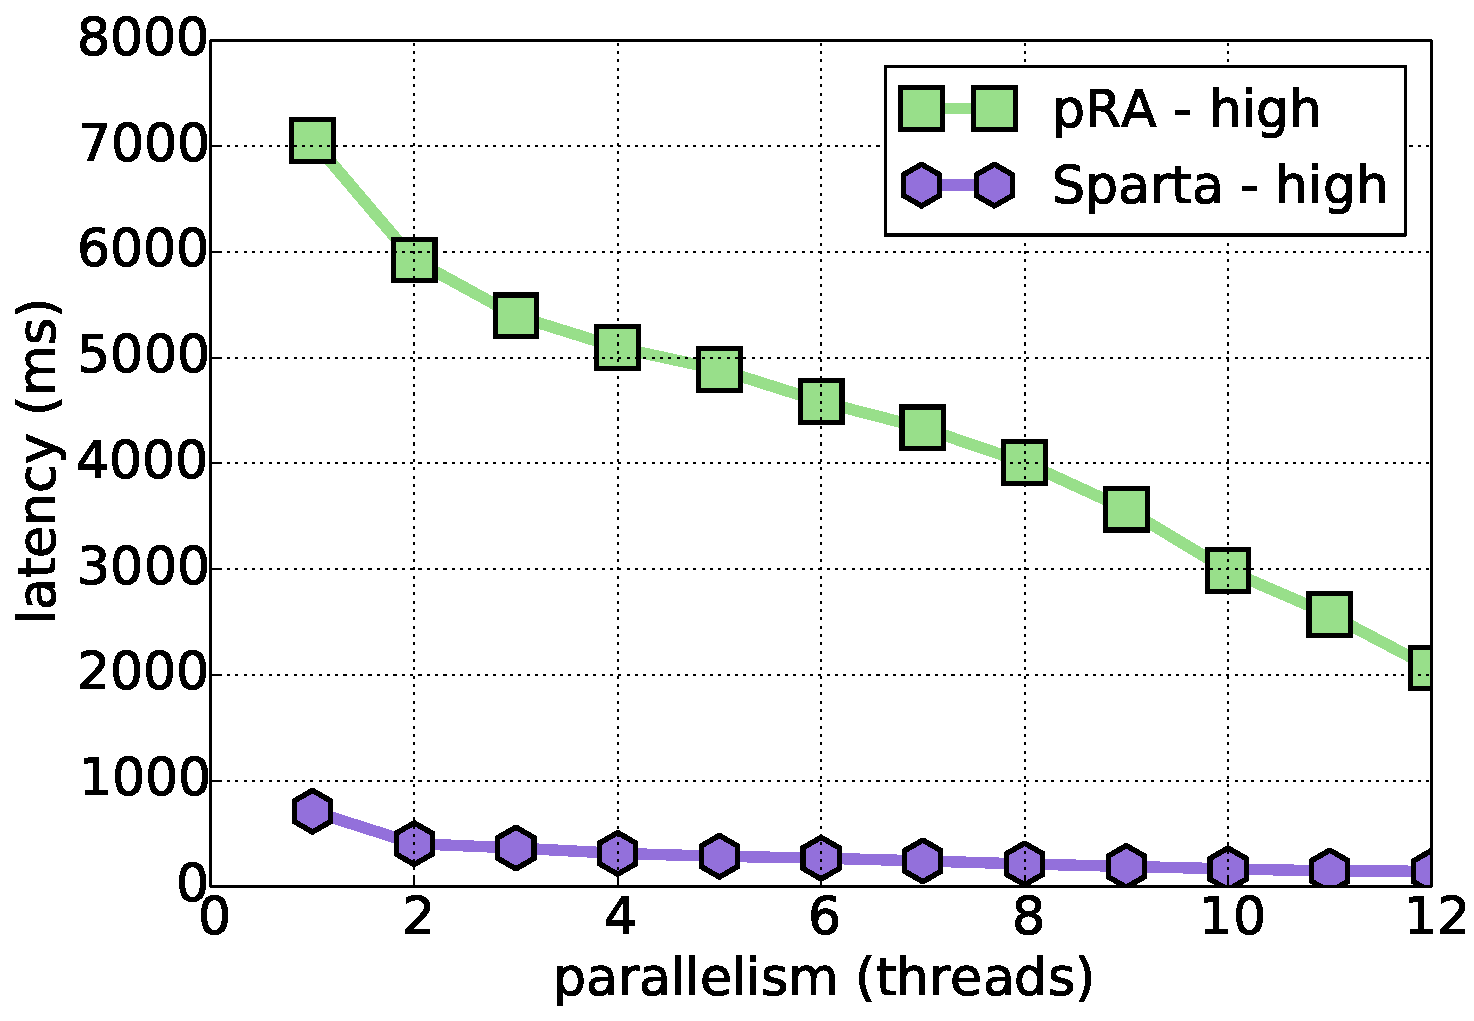
\includegraphics[width=\textwidth]{figures/latency_12terms_cluewebX10.pdf}
	  \caption{ClueWebX10}
	% \label{fig:varying-threads-12-terms}
      \end{subfigure}
\end{tabular}
}
\caption{Top-k query latency scaling with intra-query parallelism, for $12$-term queries.}
\label{fig:threads-scaling}
\end{figure}

\begin{table}[htb]
\centering
\begin{tabular}{| c | c  | c | c | c | }
\hline
   \alg\hi &  \pRA\hi & \pBMW\hi & \pBMW\lo & pJASS \\  \hline
    12.5 &  10.9 & 5.95 &  6.64 & \inred{TBD} \\ \hline
\bigdataset{
  \cwten & 9.6 & 1.8 & 0.38 & 0.42 \\
  }
\hline
\end{tabular}
\caption{Average throughput (in queries per second) of the approximate algorithms on a query distribution measured for voice queries in production. }
\label{tab:thpt}
\end{table}

{\bf Throughput.\ } Finally, we compare the throughput (in queries per second) provided by the different
algorithms. To this end, we generate a workload with the query size distribution reported in~\cite{sigir/Guy16},
where the average query length is $4.2$ (std: $2.96$), and more than $5\%$ of the queries are $10$ terms or longer.
The queries are generated as follows: we first sample a query length $\ell$ from the distribution in~\cite{sigir/Guy16}, and then 
select a query uniformly at random among all the length-$\ell$ queries in the complete set of  $1200$ AOL queries. 

Table~\ref{tab:thpt} depicts the results of running this query mix on a shared worker pool  of $12$ threads. 
Here too, \alg\/ improves over its competitors by a wide margin.
\bigdataset{
, especially on \cwten, where its throughput
is 25x that of \pBMW\hi. 
}
This  advantage is thanks to a combination of \alg's speed and lower resource utilization.
 